\documentclass[a4paper, 11pt]{article}

% Nécessaire
\usepackage[utf8]{inputenc}
\usepackage[T1]{fontenc}
\usepackage{lmodern}

% Biblio
\usepackage{natbib}
\bibliographystyle{abbrvnat}
\usepackage{hypernat}
\bibpunct{\textcolor{blue}{[}}{\textcolor{blue}{]}}{}{a}{\textcolor{blue}{,}}{;}

\usepackage[french]{babel}
\usepackage{amsmath, amsthm}
\usepackage{amsfonts,amssymb}

% Marge
\usepackage{geometry}
\geometry{margin={2.2cm ,2cm}}

% Figures, graphiques
\usepackage{graphicx}
\usepackage{epsfig}
\usepackage{caption}

% Surlignage
\usepackage{alltt}

\usepackage{xcolor}
\usepackage{soul}
\usepackage{color}
\usepackage{colortbl}

% Indicatrice
\usepackage{dsfont}

\usepackage{multirow}
\usepackage{eurosym}
\usepackage{extarrows}
\usepackage[colorlinks=true, citecolor=blue, linkcolor=.]{hyperref}

% Graphique
\usepackage{tikz}


% Titre
\title{Modèle «définitif»}
\author{}
\date{}



\begin{document}
 \maketitle

 Il comprend notamment :
 \begin{itemize}
  \item la diapause ;
  \item la pupaison en fonction de la température ;
  \item la calibration de $E_0 \times \mu_\ell$.
 \end{itemize}

Un jeu de paramètres trouvé :

\begin{center}
\begin{tabular}{lllllll}
$\gamma$ & $p_m$ & $\mu_{ER}$ & $\mu_{EH}$ & $k$ & \texttt{stock} & $E_0\times \mu_\ell$\\
0.024 & 1.000 & 0.950 & 0.041 & 0.081 & 20064 & 9.983
\end{tabular}
\end{center}

Il produit les dynamiques visibles ci-dessous :
\begin{figure}[ht]
 \centering
 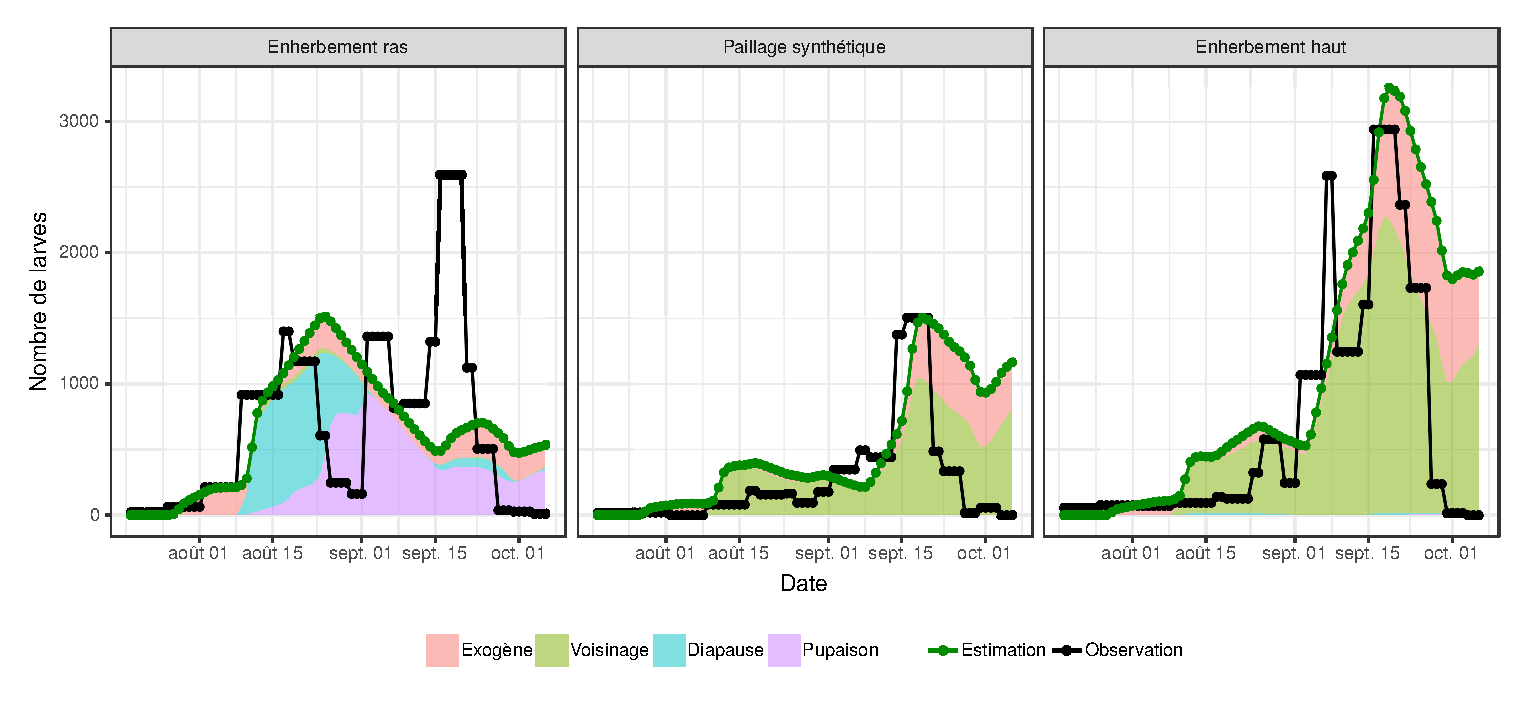
\epsfig{file = plots/REF.eps, scale = 0.65}
\end{figure}

Nombres d'individus (femelles + mâles)
\begin{center}
\begin{tabular}{llll}
 & ER & PS & EH\\
Larves (obs) & 53615 & 21097 & 53858\\
Larves (est) & 51809 & 38817 & 84659\\
Cécidomyies & 23247 & 13865 & 28495\\
Pupaison & 10075 & 0 & 50\\
Diapause & 8937 & 0 & 223\\
Voisinage & 404 & 10558 & 21601\\
Exogène & 3829 & 3306 & 6619
\end{tabular}
\end{center}

 
\end{document}
